\section{Identifying a System from Input/Output Data}

\textbf{(a)}
Put the input and output samples into the matrices
\[
X=
\begin{bmatrix}
x^{(1)}&\cdots&x^{(N)}
\end{bmatrix},
\qquad
Y=
\begin{bmatrix}
y^{(1)}&\cdots&y^{(N)}
\end{bmatrix}
\]
Then
\[
J=\sum_{k=1}^N \|Ax^{(k)}-y^{(k)}\|^2
=\|AX-Y\|_F^2
\]
The least-squares normal equation is
\[
A X X^T=Y X^T
\]
If \(X\) has full row rank, then \(XX^T\) is invertible, and the estimate is
\[
\hat A=Y X^T(XX^T)^{-1}
\]
This is the same as solving one least-squares problem for each row of \(A\).

\textbf{(b)}
For this dataset \(m=10,\quad n=3,\quad N=100\) and \(
\mathrm{rank}(X)=3
\)
so \(X\) has full row rank and \(XX^T\) is invertible.
%  The estimate is
% \[
% \hat A=
% \begin{bmatrix}
% 2.0299&5.0208&5.0104\\
% 0.0114&6.9999&1.0106\\
% 7.0424&-0.0025&6.9448\\
% 6.9977&3.9759&4.0024\\
% 9.0130&1.0449&6.9980\\
% 4.0119&3.9649&9.0267\\
% 4.9871&6.9723&8.0336\\
% 7.9425&6.0875&3.0174\\
% 0.0094&8.9722&-0.0385\\
% 1.0612&8.0208&7.0285
% \end{bmatrix}
% \]
% The RMS residual is
% \[
% \frac{\|\hat A X-Y\|_F}{\sqrt{N}}=6.453362
% \]


\begin{figure}[H]
    \centering
    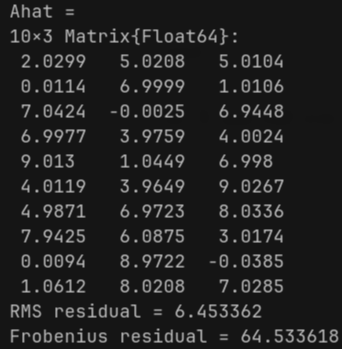
\includegraphics[width=0.4\textwidth]{img/1b.png}
\end{figure}

\subsection{Code}
\begin{lstlisting}[language={}]
using LinearAlgebra

include(joinpath(@__DIR__, "readclassjson.jl"))

data = readclassjson(joinpath(@__DIR__, "sysid_data.json"))
X = data["X"]
Y = data["Y"]

Ahat = Y * X' * inv(X * X')
residual = Ahat * X - Y
\end{lstlisting}
